\subsection{Création d'un corpus parallèle}

L'entraînement d'un modèle de traduction nécessite la présence d'un \emph{corpus parallèle}
c.-à-d. un corpus contenant les mêmes phrases dans plusieurs langues (dans notre cas, Français et Français aphasique).
Cependant, un tel corpus n'existe pas. 
Il est donc nécessaire de le créer.
La création d'un tel corpus nécessite la collecte d'un corpus de parole aphasique de taille suffisante.
Ce corpus doit être en suite traiter par des experts pour corriger les erreurs dedans.
Or, nous avons déjà établie qu'un corpus de parole aphasique de taille suffisante n'existe pas.
Ce chemin donc est infranchissable dans ce moment.

L'alternative proposée dans \cite{Smaili_Langlois_Pribil_2022} --- et celle que nous prenons --- 
est de créer un corpus synthétique.
c.--à.--d., partir d'un corpus de parole normale et le modifier pour introduire 
des erreurs similaires à celles trouvées dans la parole aphasique.

\subsubsection{Corpus de parole normale}

Nous avons utilisé le corpus \texttt{fra\_mixed100k} de 
\emph{\foreignlanguage{english}{Leipzig Corpora Collection}}~\cite{Goldhahn_Eckart_Quasthoff}.
Il s'agit d'un corpus de 100000 phrases Françaises collectées de plusieurs sites web.
Ces phrases sont diverses dans leur contenu, longueur, vocabulaire et structure grammaticale.

\subsubsection{Extraction du vocabulaire et sélection des mots à modifier}

Les erreurs causées par l'aphasie de Broca ne sont pas déterministes.
Un individu qui en souffre ne se trompe pas sur tous les mots, ni de la même manière sur le même mot.
Cependant, les erreurs ne sont pas uniformément réparties sur le vocabulaire.
Naturellement, un tel individu à tendance à se tromper plus sur les mots ``\emph{difficiles}''.
Il est aussi plus susceptible de se tromper sur les mots qu'il utilise le plus souvent.
On peut donc s'attendre à un biais pour les mots fréquents et difficiles.

Pour simuler ce biais dans notre corpus, nous avons extrait le vocabulaire du corpus.
Puis, nous avons sélectionné les mots ``\emph{difficiles}''. 
Nous avons considéré un mot ``\emph{difficile}'' s'il est long (plus de 2 syllabes).
Nous avons considéré ses mots dans l'ordre de leur fréquence dans le corpus (les 1000 premiers).

\subsubsection{Génération et filtrage des erreurs synthétiques}

Les mots sélectionnés à l'étape précédente sont donnés à chatGPT 
qui est chargé de générer 10 erreurs pour chaque mot dans le style d'un individu souffrant de l'aphasie de Broca.
Le résultat de cette opération est une liste de 10000 couples (mot, erreur).

Ces couples sont filtrés manuellement pour supprimer les erreurs trop similaires au mot original 
(par exemple celle qui en différent uniquement par la suppression d'une lettre)
et les erreurs dissimilaires à celle produite par un individu aphasique.
Cela a donné une moyenne de 5 erreurs retenues par mot.

\subsubsection{Génération des phrases erronées}

Le corpus parallèle est créé à partir du corpus original \(C\) et de l'ensemble des erreurs filtrés \(L\) 
de la façon suivante (voir Figure~\ref{fig:flow-corpus}) :

\begin{enumerate}
    \item Sélectionner de \(C\) les phrases qui contiennent au moins un mot présent dans \(L\).
    \item Pour chaque phrase sélectionnée, générer des variantes erronées en remplaçant les mots présents dans \(L\)
    par les erreurs correspondantes (si plusieurs mots existent, prendre toutes les combinaisons possibles).
    \item Insérer les phrases générées dans le corpus parallèle avec la phrase de départ comme traduction.
\end{enumerate}
\begin{figure}[hbt]
    \begin{center}
        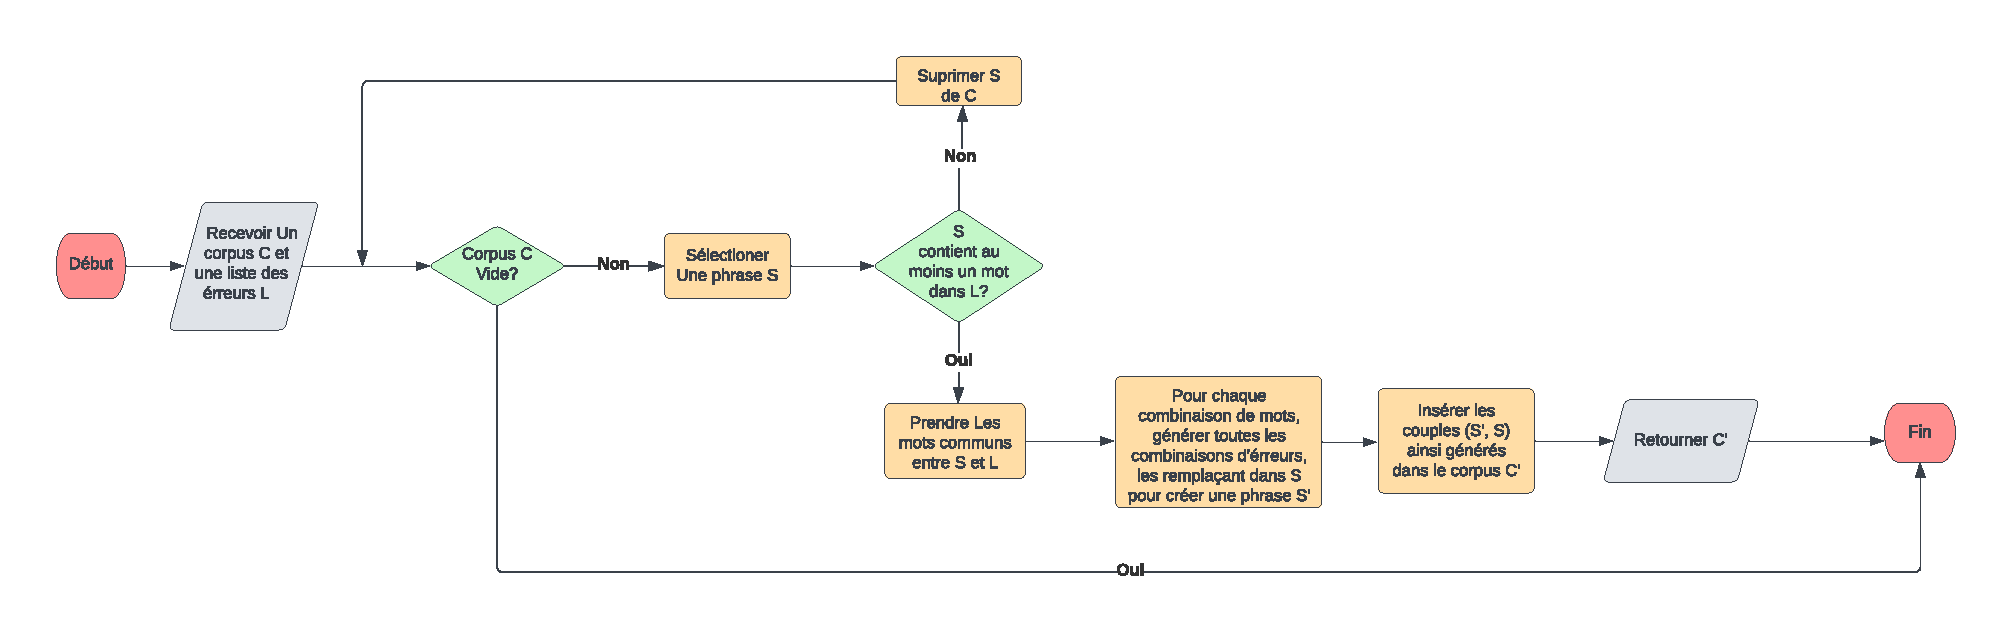
\includegraphics[width=\textwidth]{assets/pdf/flow.pdf}
    \end{center}
    \caption{Organigramme de la création du corpus parallèle.}
    \label{fig:flow-corpus}
\end{figure}
Le corpus ainsi créé compte 282689 couples de phrases.
Cela est bien suffisant pour entraîner un réseau de neurones.
L'étape de modélisation peut donc être entamée.
